\subsection{Triggers}

\subsubsection{Hadronic signal region and control samples\label{sec:signal_triggers}} 

Only events passing one or more HLT triggers based on online quantanties 
are recorded to be analyzed. For any analysis, in general, it is 
not expected that all recorded events reconstructed offline, pass the online
trigger as detector conditions, energy corrections, and object-based quantaties
differ offline. In this analysis, cross-triggers at the HLT
based on quantities \scalht and \alphat (labelled as \verb!HTxxx_AlphaT0pyy!) 
are used with various thresholds to record candidate events for the hadronic (signal)
region. In order to keep the cross-trigger's computational time low, the online quantaties
are constructed using calorimeter based jets (calo jets), and the use of
partcle-flow jets in this analysis is expected to introduce inefficiencies.

Each \scalht bin is seeded by a single trigger chosen based on the
efficiency of the trigger in that \scalht bin. The \alphat thresholds of the
\verb!HTxxx_AlphaT0pyy! triggers were tuned according to the threshold
on the \scalht leg in order to fully suppress QCD multijet events~\cite{RA1Paper2012}
and simultaneously satisfying other criteria, such as maintaining
acceptable trigger rates.



%Table~\ref{tab:htalphat-triggers} summarises the thresholds used for
%the \verb!HTxxx_AlphaT0pyy! triggers. 
%
The \verb!HTxxx_AlphaT0pyy! trigger efficiencies are measured with a
reference (\ie, unbiased) event sample recorded by an unprescaled,
loosely-isolated, eta-restricted single muon 
trigger, \verb!HLT_IsoMu24_eta2p1!, within the \verb!SingleMu! dataset. A
sample of events containing at least one isolated muon with $\pt >
25\gev$ and $|\eta| < 2.1$ is used (similar to the \mj control sample
defined in Section~\ref{sec:def-control-samples}). A cut of $\Delta
{\rm R} > 0.5$ is placed between all muons and jets in each event, and
only jets are considered in the calculation of \scalht, \mht, and
\alphat, \ie the muon is ignored.

\begin{table}[!h]
  \caption{List of signal triggers and their efficiencies (\%), as
    measured in data. The trigger efficiency is $\sim$100\% for all
    bins above $\scalht > 675\gev$.}  
  \label{tab:htalphat-triggers}
  \centering
  \footnotesize
  \begin{tabular}{ cccccc }
    \hline
    \hline
    Offline \scalht       & Offline \alphat & L1 seed (\verb!L1_?!)         & Trigger (\verb!HLT_?!)  & \multicolumn{2}{c}{Efficiency (\%)}          \\ [0.5ex]
    region (\gev)         & threshold       & (highest thresholds)          &                         & $2 \leq \njet \leq 3$ & $\njet \geq 4$       \\ [0.5ex]
    \hline
    %$200 < \scalht < 275$ & 0.65            & \verb!DoubleJetC64!           & \verb!HT200_AlphaT0p57! & $81.8^{+0.4}_{-0.4}$  & $78.9^{+0.3}_{-0.4}$ \\
    %$275 < \scalht < 325$ & 0.60            & \verb!DoubleJetC64!           & \verb!HT200_AlphaT0p57! & $95.2^{+0.3}_{-0.4}$  & $90.0^{+1.2}_{-1.3}$ \\
    %$325 < \scalht < 375$ & 0.55            & \verb!DoubleJetC64 OR HTT175! & \verb!HT300_AlphaT0p53! & $97.9^{+0.3}_{-0.3}$  & $95.6^{+0.9}_{-1.0}$ \\
    $375 < \scalht < 475$ & 0.55            & \verb!DoubleJetC64 OR HTT175! & \verb!HT300_AlphaT0p53! & $94.2^{+0.5}_{-0.6}$  & $90.5^{+1.2}_{-1.3}$ \\
    $475 < \scalht < 575$ & 0.55            & \verb!DoubleJetC64 OR HTT175! & \verb!HT350_AlphaT0p52! & $96.2^{+0.8}_{-0.9}$  & $94.6^{+1.2}_{-1.4}$ \\
    $575 < \scalht < 675$ & 0.55            & \verb!DoubleJetC64 OR HTT175! & \verb!HT400_AlphaT0p51! & $95.4^{+1.4}_{-1.8}$  & $98.7^{+0.7}_{-1.12}$ \\
    $\scalht > 675$       & 0.55            & \verb!DoubleJetC64 OR HTT175! & \verb!HT400_AlphaT0p51! & $100^{+0.0}_{-2.0}$  & $100^{+0.0}_{-2.0}$ \\
    \hline
    \hline
  \end{tabular}
\end{table}


Table~\ref{tab:htalphat-triggers} summarises the measured efficiencies
for the \verb!HTxxx_AlphaT0pyy! triggers in the relevant \scalht
bins. The trigger efficiencies are measured for both \njet
multiplicity bins. %The efficiencies are generally observed to be high,
%$\sim$100\%, except for the low \scalht region $200 < \scalht <
%325\gev$. The inefficiencies at low \scalht are mainly due to the L1
seeds for which thresholds were raised to a relatively high level in
order to maintain trigger rates in the high-pileup conditions towards
the end of Run 1. The inefficiencies are slightly larger in the higher
jet multiplicity category due to a larger number of jets summing to
the same \scalht, resulting in softer
jets. Figures~\ref{fig:eff-alphat-le3j} and~\ref{fig:eff-alphat-ge4j}
show the efficiency curves for the \verb!HTxxx_AlphaT0pyy! triggers in
the three lowest \scalht bins, for the \njetlow and \njethigh
categories, respectively. The efficiencies are also determined at the
level of event categories and no dependence on \nb is observed, with
efficiencies agreeing within statistical uncertainties.


\begin{figure}[!h]
  \begin{center}
    \subfigure[\njetlow, $375 < \scalht < 475 \gev$]{
      
\includegraphics[width=0.4\textwidth,page=30]{figures/trigger/plotDump/v29/HT375_475_100_100_50_AlphaT_HT300xaT0p53_PF_le3j_RunAtFNAL.pdf}
    }
    \subfigure[\njethigh, $375 < \scalht < 475 \gev$]{
      
\includegraphics[width=0.4\textwidth,page=30]{figures/trigger/plotDump/v29/HT375_475_100_100_50_AlphaT_HT300xaT0p53_PF_ge4j_RunAtFNAL.pdf}
    } \\
    \subfigure[\njetlow, $475 < \scalht < 525 \gev$]{
      
\includegraphics[width=0.4\textwidth,page=30]{figures/trigger/plotDump/v29/HT475_575_100_100_50_AlphaT_HT350xaT0p52_PF_le3j_RunAtFNAL.pdf}
    } 
    \subfigure[\njethigh, $475 < \scalht < 525 \gev$]{
      
\includegraphics[width=0.4\textwidth,page=30]{figures/trigger/plotDump/v29/HT475_575_100_100_50_AlphaT_HT350xaT0p52_PF_ge4j_RunAtFNAL.pdf}
    } \\
    \subfigure[\njetlow, $525 < \scalht < 675 \gev$]{
      
\includegraphics[width=0.4\textwidth,page=27]{figures/trigger/plotDump/v29/HT575_675_100_100_50_AlphaT_HT400xaT0p51_PF_ge4j_RunAtFNAL.pdf}
    }
    \subfigure[\njethigh, $525 < \scalht < 675 \gev$]{
      
\includegraphics[width=0.4\textwidth,page=27]{figures/trigger/plotDump/v29/HT575_675_100_100_50_AlphaT_HT400xaT0p51_PF_ge4j_RunAtFNAL.pdf}
    } \\
    \caption{\label{fig:eff-alphat-le3j}
      Cumulative efficiency turn-on curves for the \scalht-\alphat 
      cross triggers (as summarised in Table~\ref{tab:htalphat-triggers}) 
      that record events for the three lowest \scalht bins for events 
      satisfying \njetlow (left) and \njethigh (right). 
    }
  \end{center}
\end{figure}
%
%\begin{figure}[!h]
%  \begin{center}
%    \subfigure[Differential, $375 < \scalht < 475 \gev$]{
%      
\includegraphics[width=0.4\textwidth,page=20]{figures/trigger/plotDump/v29/HT375_475_100_100_50_AlphaT_HT300xaT0p53_PF_le3j_RunAtFNAL.pdf}
%    }
%    \subfigure[Cumulative, $375 < \scalht < 475 \gev$]{
%      
\includegraphics[width=0.4\textwidth,page=30]{figures/trigger/plotDump/v29/HT375_475_100_100_50_AlphaT_HT300xaT0p53_PF_le3j_RunAtFNAL.pdf}
%    } \\
%    \subfigure[Differential, $475 < \scalht < 525 \gev$]{
%      
\includegraphics[width=0.4\textwidth,page=20]{figures/trigger/plotDump/v29/HT475_575_100_100_50_AlphaT_HT350xaT0p52_PF_le3j_RunAtFNAL.pdf}
%    } 
%    \subfigure[Cumulative, $475 < \scalht < 525 \gev$]{
%      
\includegraphics[width=0.4\textwidth,page=30]{figures/trigger/plotDump/v29/HT475_575_100_100_50_AlphaT_HT350xaT0p52_PF_le3j_RunAtFNAL.pdf}
%    } \\
%    \subfigure[Differential, $525 < \scalht < 675 \gev$]{
%      
\includegraphics[width=0.4\textwidth,page=18]{figures/trigger/plotDump/v29/HT575_675_100_100_50_AlphaT_HT400xaT0p51_PF_le3j_RunAtFNAL.pdf}
%    }
%    \subfigure[Cumulative, $525 < \scalht < 675 \gev$]{
%      
\includegraphics[width=0.4\textwidth,page=27]{figures/trigger/plotDump/v29/HT575_675_100_100_50_AlphaT_HT400xaT0p51_PF_le3j_RunAtFNAL.pdf}
%    } \\
%    \caption{\label{fig:eff-alphat-le3j}
%      (Left) Differential and (Right) cumulative efficiency turn-on 
%      curves for the \scalht-\alphat cross triggers (as summarised in 
%      Table~\ref{tab:htalphat-triggers}) that record events for the
%      three lowest \scalht bins  for events satisfying \njetlow. 
%    }
%  \end{center}
%\end{figure}

%begin{figure}[!h]
% \begin{center}
%   \subfigure[Differential, $375 < \scalht < 475 \gev$]{
%     
\includegraphics[width=0.4\textwidth,page=20]{figures/trigger/plotDump/v29/HT375_475_100_100_50_AlphaT_HT300xaT0p53_PF_ge4j_RunAtFNAL.pdf}
%   }
%   \subfigure[Cumulative, $375 < \scalht < 475 \gev$]{
%     
\includegraphics[width=0.4\textwidth,page=30]{figures/trigger/plotDump/v29/HT375_475_100_100_50_AlphaT_HT300xaT0p53_PF_ge4j_RunAtFNAL.pdf}
%   } \\
%   \subfigure[Differential, $475 < \scalht < 525 \gev$]{
%     
\includegraphics[width=0.4\textwidth,page=20]{figures/trigger/plotDump/v29/HT475_575_100_100_50_AlphaT_HT350xaT0p52_PF_ge4j_RunAtFNAL.pdf}
%   } 
%   \subfigure[Cumulative, $475 < \scalht < 525 \gev$]{
%     
\includegraphics[width=0.4\textwidth,page=30]{figures/trigger/plotDump/v29/HT475_575_100_100_50_AlphaT_HT350xaT0p52_PF_ge4j_RunAtFNAL.pdf}
%   } \\
%   \subfigure[Differential, $525 < \scalht < 675 \gev$]{
%     
\includegraphics[width=0.4\textwidth,page=18]{figures/trigger/plotDump/v29/HT575_675_100_100_50_AlphaT_HT400xaT0p51_PF_ge4j_RunAtFNAL.pdf}
%   }
%   \subfigure[Cumulative, $525 < \scalht < 675 \gev$]{
%     
\includegraphics[width=0.4\textwidth,page=27]{figures/trigger/plotDump/v29/HT575_675_100_100_50_AlphaT_HT400xaT0p51_PF_ge4j_RunAtFNAL.pdf}
%   } \\
%   \caption{\label{fig:eff-alphat-ge4j}
%     (Left) Differential and (Right) cumulative efficiency turn-on 
%     curves for the \scalht-\alphat cross triggers (as summarised in 
%     Table~\ref{tab:htalphat-triggers}) that record events for the
%     three lowest \scalht bins  for events satisfying \njethigh. 
%   }
% \end{center}
%end{figure}
\FloatBarrier

\subsubsection{Muon and photon control samples\label{sec:muon_triggers}}

Events for the muon control sample are recorded with the \verb!HLT_IsoMu24_eta2p1! 
trigger. Figure~\ref{fig:eff-muon} (left) shows the \verb!HLT_IsoMu24_eta2p1! 
trigger efficiency as determined in bins of number of primary vertices 
for muon $\pt >$ 25 \gev and $|\eta| <$ 2.1 by the muon POG~\cite{ref:muon-eff}.
Figure~\ref{fig:eff-muon} (right) shows the disribution of the number 
of vertices in the muon control sample seeded by the \verb!HLT_IsoMu24_eta2p1!. 
The efficiency at the mean number of vertices (nVtx = 13) is taken as flat
trigger efficiency across \njet, \nb and \scalht. This measurement 
agrees well with direct tag and probe measurments in bins of 
\njet, \nb, \scalht done elsewhere. [REF]

\begin{figure}[!h]
  \begin{center}
  \subfigure{
    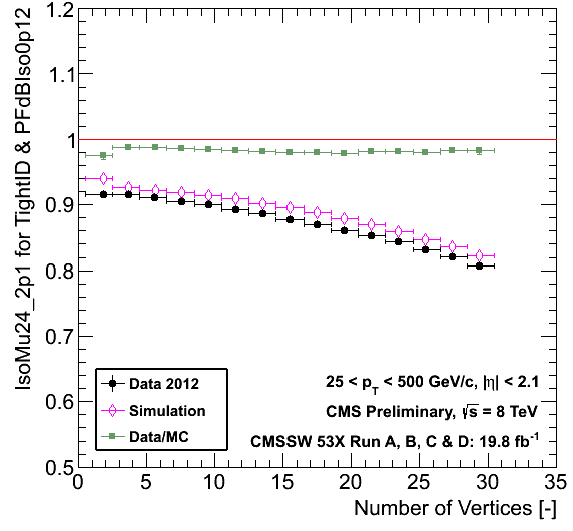
\includegraphics[width=0.3\textwidth,]{figures/trigger/muonEffvsNvtx}
    }   
  \subfigure{
   \includegraphics[width=0.42\textwidth,page=65]{figures/data-mc/v21/mu/muonLook_pfJet_ge2j_375.pdf}
   }\\     
    \caption{\label{fig:eff-muon}
    (left) Muon trigger efficiency as a function of
    number of primary vertices for muon $\pt>$ 25 \gev and
    $|\eta| <$ 2.1., (right) number of primary vertices
    in muon control sample.} 
 
  \end{center}
\end{figure}

Events for the photon control sample are recorded with the
\verb!HLT_Photon150! trigger, which is $\sim100\%$ efficient for
$E_{\rm T}^{\rm photon} > 165\gev$ and $\scalht > 375\gev$, as shown
in Figure~\ref{fig:eff-photon}. The efficiency measurement is made
using the \verb!HLT_Photon90! trigger as a reference, and we assume
that the \verb!L1_SingleEG22! seed is fully efficient.

\begin{figure}[!h]
  \begin{center}
  \subfigure[\njetlow]{
    \includegraphics[width=0.43\textwidth,page=6]{figures/trigger/g_barrel_375_caloJet_le3j_}
    }   
  \subfigure[\njethigh]{
   \includegraphics[width=0.43\textwidth,page=6]{figures/trigger/g_barrel_375_caloJet_ge4j_}
   }\\     
    \caption{\label{fig:eff-photon}
    Cumulative efficiency turn-on curves for the \texttt{HLT\_Photon150} trigger 
    as a function of photon \pt for events satisfying \njetlow 
    (left) and \njethigh (right).} 
  \end{center}
\end{figure}


\FloatBarrier



































































































%\clearpage
%\section{Triggers\label{sec:triggers}} 
%
%\subsection{Hadronic signal region\label{sec:signal_triggers}} 
%
%%Cross triggers at the HLT based on the quantities \scalht and \alphat
%%(labelled as \verb!HTxxx_AlphaT0pyy!) are used with various thresholds
%%to record candidate events for the hadronic signal region. Only a
%%single trigger is used to seed each \scalht bin of the signal region,
%%based on the \scalht threshold. The \alphat thresholds of the
%%\verb!HTxxx_AlphaT0pyy! triggers are tuned according to the threshold
%%on the \scalht leg in order to fully suppress QCD multijet events
%%(whilst simultaneously satisfying other criteria, such as maintaining
%%acceptable trigger rates).
%%
%%The \verb!HT200_Alphat0p57! trigger recorded candidate signal events
%%in the \verb!ParkedHTMHT! dataset, which was introduced at the
%%beginning of Run B in 2012. All other triggers were available in
%%Stream A from the start of Run 1 and seed the \verb!HTMHT! dataset.
%%
%%Table~\ref{tab:htalphat-triggers} summarises the thresholds used for
%%the \verb!HTxxx_AlphaT0pyy! triggers. Also listed are the Level-1
%%trigger seeds and thresholds. \verb!FastJet! corrections are applied
%%to the input jets for all HLT triggers. To ensure that the \scalht leg
%%of each \verb!HTxxx_AlphaT0pyy! trigger is efficient for the signal
%%region selection criteria, the lower bounds of the offline \scalht
%%bins are offset by 25\GeV with respect to the trigger \scalht
%%thresholds.
%%
%%The \verb!HTxxx_AlphaT0pyy! trigger efficiencies are measured with a
%%reference (\ie, unbiased) event sample recorded by an unprescaled,
%%loosely-isolated, eta-restricted single muon trigger,
%%\verb!HLT_IsoMu24_eta2p1!, within the \verb!SingleMu! dataset. A
%%sample of events containing at least one isolated muon with $\pt >
%%25\gev$ and $|\eta| < 2.1$ is used (similar to the \mj control sample
%%defined in Section~\ref{sec:def-control-samples}). A cut of $\Delta
%%{\rm R} > 0.5$ is placed between all muons and jets in each event, and
%%only jets are considered in the calculation of \scalht, \mht, and
%%\alphat, \ie the muon is ignored.
%%
%%Table~\ref{tab:htalphat-triggers} summarises the measured efficiencies
%%for the \verb!HTxxx_AlphaT0pyy! triggers in the relevant \scalht
%%bins. The trigger efficiencies are measured for both \njet
%%multiplicity bins. The efficiencies are generally observed to be high,
%%$\sim$100\%, except for the low \scalht region $200 < \scalht <
%%325\gev$. The inefficiencies at low \scalht are mainly due to the L1
%%seeds for which thresholds were raised to a relatively high level in
%%order to maintain trigger rates in the high-pileup conditions towards
%%the end of Run 1. The inefficiencies are slightly larger in the higher
%%jet multiplicity category due to a larger number of jets summing to
%%the same \scalht, resulting in softer
%%jets. Figures~\ref{fig:eff-alphat-le3j} and~\ref{fig:eff-alphat-ge4j}
%%show the efficiency curves for the \verb!HTxxx_AlphaT0pyy! triggers in
%%the three lowest \scalht bins, for the \njetlow and \njethigh
%%categories, respectively. The efficiencies are also determined at the
%%level of event categories and no dependence on \nb is observed, with
%%efficiencies agreeing within statistical uncertainties.
%%
%%%\fixme{Various cross-checks were performed, by comparing efficiencies
%%%  measured from different sub-samples, such as: exactly one isolated
%%%  muon versus at least two isolated muons (W-enriched versus
%%%  DY-enriched); exactly zero b-tagged jets versus at least one
%%%  b-tagged jet (W-enriched versus \ttbar-enriched); the nominal choice
%%%  of $\mht/\met < 1.25$ versus one in which this criterion is
%%%  inverted\footnote{This cross-check concerns the QCD multijet
%%%    background estimation method, that relies on a $\mht/met$ data
%%%    sideband, as described in Section~\ref{sec:qcd}} ($\mht/\met >
%%%  1.25$). For all cross-checks, the efficiencies were agreed within
%%%  statistical uncertainties for \scalht and \alphat values above the
%%%  trigger thresholds.}
%%
%%\begin{table}[!h]
%%  \caption{List of signal triggers and their efficiencies (\%), as
%%    measured in data. The trigger efficiency is $\sim$100\% for all
%%    bins above $\scalht > 475\gev$.}  
%%  \label{tab:htalphat-triggers}
%%  \centering
%%  \footnotesize
%%  \begin{tabular}{ cccccc }
%%    \hline
%%    \hline
%%    Offline \scalht       & Offline \alphat & L1 seed (\verb!L1_?!)         & Trigger (\verb!HLT_?!)  & \multicolumn{2}{c}{Efficiency (\%)}          \\ [0.5ex]
%%    region (\gev)         & threshold       & (highest thresholds)          &                         & $2 \leq \njet \leq 3$ & $\njet \geq 4$       \\ [0.5ex]
%%    \hline
%%    $200 < \scalht < 275$ & 0.65            & \verb!DoubleJetC64!           & \verb!HT200_AlphaT0p57! & $81.8^{+0.4}_{-0.4}$  & $78.9^{+0.3}_{-0.4}$ \\
%%    $275 < \scalht < 325$ & 0.60            & \verb!DoubleJetC64!           & \verb!HT200_AlphaT0p57! & $95.2^{+0.3}_{-0.4}$  & $90.0^{+1.2}_{-1.3}$ \\
%%    $325 < \scalht < 375$ & 0.55            & \verb!DoubleJetC64 OR HTT175! & \verb!HT300_AlphaT0p53! & $97.9^{+0.3}_{-0.3}$  & $95.6^{+0.9}_{-1.0}$ \\
%%    $375 < \scalht < 475$ & 0.55            & \verb!DoubleJetC64 OR HTT175! & \verb!HT350_AlphaT0p52! & $99.2^{+0.2}_{-0.2}$  & $98.7^{+0.5}_{-0.7}$ \\
%%    $\scalht > 475$       & 0.55            & \verb!DoubleJetC64 OR HTT175! & \verb!HT400_AlphaT0p51! & $99.8^{+0.1}_{-0.3}$  & $99.6^{+0.3}_{-0.7}$ \\
%%    \hline
%%    \hline
%%  \end{tabular}
%%\end{table}
%%
%%%\clearpage
%%%\begin{figure}[!h]
%%%  \begin{center}
%%%    \subfigure[$\njetlow,   275 < \scalht < 325 \gev$]{
%%%      \includegraphics[width=0.4\textwidth]{figures/cms}
%%%    }
%%%    \subfigure[$\njethigh,   275 < \scalht < 325 \gev$]{
%%%      \includegraphics[width=0.4\textwidth]{figures/cms}
%%%    } \\
%%%    \subfigure[$\njetlow,   325 < \scalht < 375 \gev$]{
%%%      \includegraphics[width=0.4\textwidth]{figures/cms}
%%%    } 
%%%    \subfigure[$\njethigh,   325 < \scalht < 375 \gev$]{
%%%      \includegraphics[width=0.4\textwidth]{figures/cms}
%%%    } \\
%%%    \subfigure[$\njetlow,   375 < \scalht < 475 \gev$]{
%%%      \includegraphics[width=0.4\textwidth]{figures/cms}
%%%    }
%%%    \subfigure[$\njethigh,   375 < \scalht < 475 \gev$]{
%%%      \includegraphics[width=0.4\textwidth]{figures/cms}
%%%    } \\
%%%    \caption{\label{fig:eff-alphat-diff}Efficiency turn-on
%%%      curve for the \scalht-\alphat cross trigger and \scalht bin
%%%      (paired as defined in Table~\ref{tab:htalphat-triggers}) for
%%%      events satisfying (left)
%%%      \njetlow and (right) \njethigh. }
%%%  \end{center}
%%%\end{figure}
%%
%\begin{figure}[!h]
%  \begin{center}
%    \subfigure[Differential, $375 < \scalht < 475 \gev$]{
%      
\includegraphics[width=0.4\textwidth,page=20]{figures/trigger/plotDump/v28/HT375_475_100_100_50_AlphaT_HT250xaT0p55_PF_le3j_RunAtFNAL.pdf}
%    }
%    \subfigure[Cumulative, $375 < \scalht < 475 \gev$]{
%      
\includegraphics[width=0.4\textwidth,page=30]{figures/trigger/plotDump/v28/HT375_475_100_100_50_AlphaT_HT250xaT0p55_PF_le3j_RunAtFNAL.pdf}
%    } \\
%    \subfigure[Differential, $475 < \scalht < 525 \gev$]{
%      
\includegraphics[width=0.4\textwidth,page=20]{figures/trigger/plotDump/v28/HT475_575_100_100_50_AlphaT_HT300xaT0p53_PF_le3j_RunAtFNAL.pdf}
%    } 
%    \subfigure[Cumulative, $475 < \scalht < 525 \gev$]{
%      
\includegraphics[width=0.4\textwidth,page=30]{figures/trigger/plotDump/v28/HT475_575_100_100_50_AlphaT_HT300xaT0p53_PF_le3j_RunAtFNAL.pdf}
%    } \\
%    \subfigure[Differential, $525 < \scalht < 675 \gev$]{
%      
\includegraphics[width=0.4\textwidth,page=20]{figures/trigger/plotDump/v28/HT575_675_100_100_50_AlphaT_HT350xaT0p52_PF_le3j_RunAtFNAL.pdf}
%    }
%    \subfigure[Cumulative, $525 < \scalht < 675 \gev$]{
%      
\includegraphics[width=0.4\textwidth,page=30]{figures/trigger/plotDump/v28/HT575_675_100_100_50_AlphaT_HT350xaT0p52_PF_le3j_RunAtFNAL.pdf}
%    } \\
%    \caption{\label{fig:eff-alphat-le3j}
%      (Left) Differential and (Right) cumulative efficiency turn-on 
%      curves for the \scalht-\alphat cross triggers (as summarised in 
%      Table~\ref{tab:htalphat-triggers}) that record events for the
%      three lowest \scalht bins  for events satisfying \njetlow. 
%    }
%  \end{center}
%\end{figure}
%%
%%\begin{figure}[!h]
%%  \begin{center}
%%    \subfigure[Differential, $200 < \scalht < 275 \gev$]{
%%      \includegraphics[width=0.4\textwidth,page=11]{figures/trigger/HT200_275_73_73_36_AlphaT_ge4j_RunAtFNAL}
%%    }
%%    \subfigure[Cumulative, $200 < \scalht < 275 \gev$]{
%%      \includegraphics[width=0.4\textwidth,page=18]{figures/trigger/HT200_275_73_73_36_AlphaT_ge4j_RunAtFNAL}
%%    } \\
%%    \subfigure[Differential, $275 < \scalht < 325 \gev$]{
%%      \includegraphics[width=0.4\textwidth,page=11]{figures/trigger/HT275_325_73_73_36_AlphaT_ge4j_RunAtFNAL}
%%    } 
%%    \subfigure[Cumulative, $275 < \scalht < 325 \gev$]{
%%      \includegraphics[width=0.4\textwidth,page=18]{figures/trigger/HT275_325_73_73_36_AlphaT_ge4j_RunAtFNAL}
%%    } \\
%%    \subfigure[Differential, $325 < \scalht < 375 \gev$]{
%%      \includegraphics[width=0.4\textwidth,page=11]{figures/trigger/HT325_375_86_86_43_AlphaT_ge4j_RunAtFNAL}
%%    }
%%    \subfigure[Cumulative, $325 < \scalht < 375 \gev$]{
%%      \includegraphics[width=0.4\textwidth,page=18]{figures/trigger/HT325_375_86_86_43_AlphaT_ge4j_RunAtFNAL}
%%    } \\
%%    \caption{\label{fig:eff-alphat-ge4j}
%%      (Left) Differential and (Right) cumulative efficiency turn-on 
%%      curves for the \scalht-\alphat cross triggers (as summarised in 
%%      Table~\ref{tab:htalphat-triggers}) that record events for the
%%      three lowest \scalht bins  for events satisfying \njethigh. 
%%    }
%%  \end{center}
%%\end{figure}
%%
%%%\begin{figure}[!h]
%%%  \begin{center}
%%%    \subfigure[$\njetlow,   275 < \scalht < 325 \gev$]{
%%%      \includegraphics[width=0.4\textwidth]{figures/cms}
%%%    }
%%%    \subfigure[$\njetlow,   275 < \scalht < 325 \gev$]{
%%%      \includegraphics[width=0.4\textwidth]{figures/cms}
%%%    } \\
%%%    \subfigure[$\njetlow,   325 < \scalht < 375 \gev$]{
%%%      \includegraphics[width=0.4\textwidth]{figures/cms}
%%%    } 
%%%    \subfigure[$\njetlow,   325 < \scalht < 375 \gev$]{
%%%      \includegraphics[width=0.4\textwidth]{figures/cms}
%%%    } \\
%%%    \subfigure[$\njetlow,   375 < \scalht < 475 \gev$]{
%%%      \includegraphics[width=0.4\textwidth]{figures/cms}
%%%    }
%%%    \subfigure[$\njetlow,   375 < \scalht < 475 \gev$]{
%%%      \includegraphics[width=0.4\textwidth]{figures/cms}
%%%    } \\
%%%    \caption{\label{fig:eff-alphat-diff-le3j}Left: distribution of the
%%%      \alphat variable in a given \scalht bin after applying the event
%%%      selection described in the text, for events collected with the
%%%      \texttt{IsoMu24\_eta2p1} trigger (red histogram) and the
%%%      \scalht-\alphat cross-trigger (black histogram). The
%%%      \scalht-\alphat cross-trigger used for each \scalht bin is
%%%      defined in Table~\ref{tab:htalphat-triggers}. Right: resulting
%%%      efficiency turn-on curve for the given \scalht-\alphat
%%%      cross-trigger and \scalht bin. All plots are constructed for the
%%%      \njetlow multiplicity bin.}
%%%  \end{center}
%%%\end{figure}
%%
%%%\begin{figure}[!h]
%%%  \begin{center}
%%%    \subfigure[$\njethigh,   275 < \scalht < 325 \gev$]{
%%%      \includegraphics[width=0.4\textwidth]{figures/cms}
%%%    }
%%%    \subfigure[$\njethigh,   275 < \scalht < 325 \gev$]{
%%%      \includegraphics[width=0.4\textwidth]{figures/cms}
%%%    } \\
%%%    \subfigure[$\njethigh,   325 < \scalht < 375 \gev$]{
%%%      \includegraphics[width=0.4\textwidth]{figures/cms}
%%%    } 
%%%    \subfigure[$\njethigh,   325 < \scalht < 375 \gev$]{
%%%      \includegraphics[width=0.4\textwidth]{figures/cms}
%%%    } \\
%%%    \subfigure[$\njethigh,   375 < \scalht < 475 \gev$]{
%%%      \includegraphics[width=0.4\textwidth]{figures/cms}
%%%    }
%%%    \subfigure[$\njethigh,   375 < \scalht < 475 \gev$]{
%%%      \includegraphics[width=0.4\textwidth]{figures/cms}
%%%    } \\
%%%    \caption{\label{fig:eff-alphat-diff-ge4j}Left: distribution of the
%%%      \alphat variable in a given \scalht bin after applying the event
%%%      selection described in the text, for events collected with the
%%%      \texttt{IsoMu24\_eta2p1} trigger (red histogram) and the
%%%      \scalht-\alphat cross-trigger (black histogram). The
%%%      \scalht-\alphat cross-trigger used for each \scalht bin is
%%%      defined in Table~\ref{tab:htalphat-triggers}. Right: resulting
%%%      efficiency turn-on curve for the given \scalht-\alphat
%%%      cross-trigger and \scalht bin. All plots are constructed for the
%%%      \njethigh multiplicity bin.}
%%%  \end{center}
%%%\end{figure}
%
%%\subsection{Hadronic control sample\label{sec:had_control_triggers}} 
%%
%%Prescaled \scalht triggers, labelled henceforth as \verb!HTxxx!, are
%%used with various thresholds to record events for the hadronic control
%%region.
%%Only a single trigger is used to seed each \scalht bin of the hadronic
%%control sample, based on the \scalht threshold, \ie the same approach
%%as used by the signal triggers. As a consequence, the \scalht
%%thresholds of 200, 250, 300, 350, and 400\gev for the \verb!HTxxx! and
%%\verb!HTxxx_AlphaT0pyy! triggers generally match for a given \scalht
%%bin in the signal region and hadronic control sample.
%%
%%Table~\ref{tab:ht-triggers} summarises the thresholds used for both
%%the \verb!HTxxx! triggers, respectively. Also listed are the Level-1
%%seeds, which are identical to the ones used for the signal triggers,
%%and the typical (HLT) prescales value used towards the end of Run 1
%%that control the rates to the level of $\sim$1~Hz per trigger. As in
%%the case of the signal triggers, the lower bounds of the \scalht bins
%%in the hadronic control sample are shifted by 25\gev with respect to
%%the \verb!HTxxx! trigger thresholds.
%%
%%As for the signal triggers, the \verb!HTxxx! trigger efficiencies are
%%measured using the same reference event sample recorded by the
%%\verb!HLT_IsoMu24_eta2p1! trigger. The same offline selection criteria
%%are applied to the sample of events containing at least one isolated
%%muon and jets. The muon(s) is(are) ignored in the calculation of
%%\scalht. 
%%
%%A second reference sample of events, recorded with the
%%\verb!HLT_Physics! minimum bias trigger, was used to cross-check the
%%efficiency measurements from the \mj sample. Both samples are expected
%%to provide unbiased measurements of the \verb!HTxxx! trigger
%%efficiencies and indeed the resulting measurements agree within
%%statistical uncertainties. Due to the limited size of both reference
%%samples, a weighted mean of the measured efficiencies is determined.
%%Table~\ref{tab:ht-triggers} summarises these efficiencies for the
%%\verb!HTxxx! triggers for the relevant bins in \scalht. Again, the
%%trigger efficiencies are measured for the two exclusive \njet
%%multiplicity bins.
%%%Similarly, Figs.~\ref{fig:eff-alphat-diff-le3j}
%%%and~\ref{fig:eff-ht-diff-ge4j} show the efficiency curves for the
%%%(prescaled) \verb!HTxxx! triggers in the three lowest \scalht bins,
%%%for the \njetlow and \njethigh categories, respectively. 
%%
%%For the \verb!HTxxx! triggers, a (non-deterministic) prescale is
%%applied at the HLT to maintain rate. The trigger logic only accepts
%%1$/P$ triggered events, where $P$ is the prescale value. This
%%(non-deterministic) logic introduces a random element that allows
%%measurements of the trigger efficiency to fluctuate above 100\% while
%%being statistically compatible with 100\%. Any meaurement will tend to
%%100\% eith increasing sample size, and cannot fluctuate above 100\%
%%for an unprescaled \verb!HTxxx! trigger. The measurements in
%%Table~\ref{tab:ht-triggers} are consistent with this behaviour: all
%%measurements are statistically compatible with 100\% and no
%%measurement fluctuates above 100\% for the region $\scalht >
%%775\gev$. The only exception is the measurement for the bin
%%(\njet,\scalht) = (2-3,200-275\gev) appears to be significantly below
%%100\%, which is also expected given the aforementioned inefficiencies
%%at Level-1. 
%%
%%While the efficiency measurements in Table~\ref{tab:ht-triggers} have
%%large statistical uncertainties, this limitation does not impact
%%significantly the multjet background estimation method, described in
%%Section~\ref{sec:qcd}, as the method relies on ratios of data yields
%%recorded by the same \verb!HTxxx!  trigger. Regardless, the
%%statistical uncertainties on the efficiencies are folded into the
%%method. 
%%
%%Finally, Table~\ref{tab:ht-triggers} also quotes ``\scalht leg signal
%%efficiencies'', which correspond to the \htalphat signal trigger
%%efficiency on the \alphat plateau (for \alphat threhold values of
%%0.70, 0.65, and 0.60 for the \scalht regions 200--275, 275--325, and
%%$>$325\gev, respectively). As discussed previously, any significant
%%inefficiency for the signal triggers is thought to arise from the slow
%%efficiency turn on for the \scalht leg due to the high thresholds used
%%for the L1 seeds; by comparison the efficiency turn on for the \alphat
%%leg is sharp. Hence, by measuring the signal trigger efficiency on the
%%\alphat efficiency plateau, it is thought that the inefficiency on the
%%\scalht leg can be isolated and compared with the efficiency
%%measurements for the \httrigger triggers. Indeed, the two sets of
%%measurements agree within statistical uncertainties and significant
%%inefficiencies are observed only for the lowest \scalht bins.
%%
%%\begin{table}[!h]
%%  \caption{List of \texttt{HTxxx} triggers and their efficiencies
%%    (\%), as measured in data. For the ``\scalht leg signal
%%    eff.'' columns, see text for further details.}
%%  \label{tab:ht-triggers}
%%  \centering
%%  \scriptsize
%%  \begin{tabular}{ ccccllll }
%%    \hline
%%    \hline
%%    Offline \scalht & L1 seed (\verb!L1_?!) & Trigger (\verb!HLT_?!) &    Typical & \multicolumn{2}{c}{Efficiency (\%)} &    \multicolumn{2}{c}{\scalht leg signal eff. (\%)} \\ [0.5ex]
%%   region (\gev) & (highest thresholds) &  & prescale & \multicolumn{1}{c}{$2 \leq \njet \leq 3$} & \multicolumn{1}{c}{$\njet \geq 4$} & \multicolumn{1}{c}{$2 \leq \njet \leq 3$} & \multicolumn{1}{c}{$\njet \geq 4$} \\ [0.5ex]
%%
%%    \hline                                                                                     
%%    $200 < \scalht < 275$  & \verb!DoubleJetC64!           & \verb!HT250! & 4800     & $\phantom{1}66.4 \pm 14.1$                & $154.3 \pm 154.3$                     & $\phantom{1}81.9 \pm \phantom{1}0.4$ & $\phantom{1}88.5 \pm \phantom{1}0.4$ \\
%%    $275 < \scalht < 325$  & \verb!DoubleJetC64 OR HTT175! & \verb!HT250! & 2400     & $\phantom{1}97.3 \pm 23.0$                & $\phantom{1}91.7 \pm \phantom{1}53.1$ & $\phantom{1}95.2 \pm \phantom{1}0.4$ & $\phantom{1}93.8 \pm \phantom{1}1.2$ \\
%%    $325 < \scalht < 375$  & \verb!DoubleJetC64 OR HTT175! & \verb!HT300! & 1200     & $\phantom{1}79.5 \pm 20.6$                & $198.1 \pm \phantom{1}81.2$           & $\phantom{1}98.0 \pm \phantom{1}0.3$ & $\phantom{1}95.9 \pm \phantom{1}1.2$ \\
%%    $375 < \scalht < 475$  & \verb!DoubleJetC64 OR HTT175! & \verb!HT350! & 600      & $108.7 \pm 18.7$                          & $\phantom{1}54.5 \pm \phantom{1}31.6$ & $\phantom{1}99.5 \pm \phantom{1}0.2$ & $\phantom{1}99.4 \pm \phantom{1}0.4$ \\
%%    $475 < \scalht < 575$  & \verb!DoubleJetC64 OR HTT175! & \verb!HT450! & 150      & $110.6 \pm 15.9$                          & $106.4 \pm \phantom{1}26.8$           & $100.0 \pm \phantom{1}0.3$ & $100.0 \pm \phantom{1}1.1$ \\
%%    $575 < \scalht < 675$  & \verb!DoubleJetC64 OR HTT175! & \verb!HT550! & 70       & $\phantom{1}96.1 \pm 14.7$                & $104.4 \pm \phantom{1}23.1$           & $100.0 \pm \phantom{1}1.0$ & $100.0 \pm \phantom{1}2.5$ \\
%%    $675 < \scalht < 775$  & \verb!DoubleJetC64 OR HTT175! & \verb!HT650! & 25       & $\phantom{1}94.3 \pm 15.4$                & $101.2 \pm \phantom{1}21.5$           & $100.0 \pm \phantom{1}3.4$ & $100.0 \pm \phantom{1}9.8$ \\
%%    $775 < \scalht < 875$  & \verb!DoubleJetC64 OR HTT175! & \verb!HT750! & 1        & $\phantom{1}96.9 \pm \phantom{1}6.1$      & $\phantom{1}94.4 \pm \phantom{11}8.3$ & $100.0 \pm \phantom{1}7.1$ & $100.0 \pm 53.5$ \\
%%    $875 < \scalht < 975$  & \verb!DoubleJetC64 OR HTT175! & \verb!HT750! & 1        & $100.0 \pm \phantom{1}8.4$                & $100.0 \pm \phantom{1}12.6$           & $100.0 \pm 19.8$ & $100.0 \pm 60.0$ \\
%%    $975 < \scalht < 1075$ & \verb!DoubleJetC64 OR HTT175! & \verb!HT750! & 1        & $100.0 \pm 11.2$                          & $100.0 \pm \phantom{1}15.3$           & $100.0 \pm 30.0$ & $100.0 \pm 70.0$ \\
%%    $\scalht > 1075$       & \verb!DoubleJetC64 OR HTT175! & \verb!HT750! & 1        & $100.0 \pm 15.0$                          & $100.0 \pm \phantom{1}22.9$           & $100.0 \pm 40.0$ & $100.0 \pm 80.0$ \\
%%    \hline
%%    \hline                   
%%  \end{tabular}              
%%\end{table}
%%
%%%\clearpage
%%%\begin{figure}[!h]
%%%  \begin{center}
%%%    \subfigure[$\njetlow,   275 < \scalht < 325 \gev$]{
%%%      \includegraphics[width=0.4\textwidth]{figures/cms}
%%%    }
%%%    \subfigure[$\njetlow,   275 < \scalht < 325 \gev$]{
%%%      \includegraphics[width=0.4\textwidth]{figures/cms}
%%%    } \\
%%%    \subfigure[$\njetlow,   325 < \scalht < 375 \gev$]{
%%%      \includegraphics[width=0.4\textwidth]{figures/cms}
%%%    } 
%%%    \subfigure[$\njetlow,   325 < \scalht < 375 \gev$]{
%%%      \includegraphics[width=0.4\textwidth]{figures/cms}
%%%    } \\
%%%    \subfigure[$\njetlow,   375 < \scalht < 475 \gev$]{
%%%      \includegraphics[width=0.4\textwidth]{figures/cms}
%%%    }
%%%    \subfigure[$\njetlow,   375 < \scalht < 475 \gev$]{
%%%      \includegraphics[width=0.4\textwidth]{figures/cms}
%%%    } \\
%%%    \caption{\label{fig:eff-ht-diff-le3j}Left: distribution of the
%%%      \scalht variable in a given \scalht bin after applying the event
%%%      selection described in the text, for events collected with the
%%%      \texttt{IsoMu24\_eta2p1} trigger (red histogram) and the \scalht
%%%      trigger (black histogram). The \scalht trigger used for each
%%%      \scalht bin is defined in Table~\ref{tab:ht-triggers}. Right:
%%%      resulting efficiency turn-on curve for the given \scalht trigger
%%%      and \scalht bin. Note that the \scalht triggers are heavily
%%%      prescaled and so large weights and fluctuations are
%%%      observed. All plots are constructed for the \njetlow
%%%      multiplicity bin.}
%%%  \end{center}
%%%\end{figure}
%%
%%%\begin{figure}[!h]
%%%  \begin{center}
%%%    \subfigure[$\njethigh,   275 < \scalht < 325 \gev$]{
%%%      \includegraphics[width=0.4\textwidth]{figures/cms}
%%%    }
%%%    \subfigure[$\njethigh,   275 < \scalht < 325 \gev$]{
%%%      \includegraphics[width=0.4\textwidth]{figures/cms}
%%%    } \\
%%%    \subfigure[$\njethigh,   325 < \scalht < 375 \gev$]{
%%%      \includegraphics[width=0.4\textwidth]{figures/cms}
%%%    } 
%%%    \subfigure[$\njethigh,   325 < \scalht < 375 \gev$]{
%%%      \includegraphics[width=0.4\textwidth]{figures/cms}
%%%    } \\
%%%    \subfigure[$\njethigh,   375 < \scalht < 475 \gev$]{
%%%      \includegraphics[width=0.4\textwidth]{figures/cms}
%%%    }
%%%    \subfigure[$\njethigh,   375 < \scalht < 475 \gev$]{
%%%      \includegraphics[width=0.4\textwidth]{figures/cms}
%%%    } \\
%%%    \caption{\label{fig:eff-ht-diff-ge4j}Left: distribution of the
%%%      \scalht variable in a given \scalht bin after applying the event
%%%      selection described in the text, for events collected with the
%%%      \texttt{IsoMu24\_eta2p1} trigger (red histogram) and the \scalht
%%%      trigger (black histogram). The \scalht trigger used for each
%%%      \scalht bin is defined in Table~\ref{tab:ht-triggers}. Right:
%%%      resulting efficiency turn-on curve for the given \scalht trigger
%%%      and \scalht bin. Note that the \scalht triggers are heavily
%%%      prescaled and so large weights and fluctuations are
%%%      observed. All plots are constructed for the \njethigh
%%%      multiplicity bin.}
%%%  \end{center}
%%%\end{figure}
%
%\subsection{Muon control samples\label{sec:muon_triggers}}
%
%%The procedure to determine the muon trigger efficiency follows the
%%recommendations of the muon POG~\cite{ref:muon-eff}. Events for the
%%\mj and \mmj control samples are recorded with a loosely-isolated,
%%$\eta$-restricted muon trigger \verb!HLT_IsoMu24_eta2p1!. The muon
%%trigger efficiency is determined for each of the \mj and \mmj control
%%samples according to the binning scheme in \njet and \scalht. Events
%%with muons satisfying the acceptance requirements $\pt > 25\gev$ and
%%$|\eta| < 2.1$ are considered.
%%
%%The \verb!HLT_IsoMu24_eta2p1! trigger efficiency is determined from
%%data in bins of muon $\pt$ and $|\eta|$ by the muon POG from a
%%tag-and-probe method~\cite{ref:muon-eff}. These efficiencies are
%%weighted by MC yields binned according to the muon $\pt$ and $|\eta|$
%%in order to determine a single weighted efficiency measurement per
%%(\njet,\scalht) bin. Simulation-to-data scale factors for muon
%%identification and isolation efficiencies are applied to MC
%%events. These scale factors are also determined by the muon POG in
%%bins of muon $\pt$ and $|\eta|$. Table~\ref{tab:muon-effs} summarises
%%the muon trigger efficiencies which are assumed to have a relative
%%systematic uncertainty of 1\%~\cite{ref:muon-eff}. Efficiencies are
%%higher for the \mmj sample due to the fact that both muons must
%%satisfy $\pt > 30\gev$ and so can be the source of the positive
%%trigger decision. A further consequence of these thresholds
%%requirements is that there is little dependence on \scalht. 
%%
%%\begin{table}[!h]
%%  \caption{Muon trigger efficiencies (\%). Statistical uncertainties
%%    are at the per-mille level, while a relative systematic
%%    uncertainty on all measurements is assumed to be 1\%.}  
%%  \label{tab:muon-effs}
%%  \centering
%%  \footnotesize
%%  \begin{tabular}{ cccccc }
%%    \hline
%%    \hline
%%    \scalht (GeV) \textbackslash \njet & \multicolumn{2}{c}{\mj} & \multicolumn{2}{c}{\mmj} \\ [0.5ex]
%%                                       & 2-3                     & $\geq$4 & 2-3 & $\geq$4  \\ [0.5ex]
%%    \hline
%%%    200--275  & 89.1 & 89.8 & 98.9 & 98.8 \\
%%%    275--325  & 89.3 & 89.8 & 98.9 & 98.8 \\
%%%    325--375  & 89.5 & 90.0 & 98.9 & 98.8 \\
%%%    375--475  & 89.7 & 90.3 & 98.9 & 98.9 \\
%%%    475--575  & 89.8 & 90.5 & 98.9 & 98.9 \\
%%%    575--675  & 90.0 & 90.6 & 98.9 & 98.9 \\
%%%    675--775  & 90.1 & 90.7 & 99.0 & 98.9 \\
%%%    775--875  & 90.2 & 90.8 & 98.9 & 98.9 \\
%%%    875--975  & 90.4 & 90.6 & 99.0 & 98.9 \\
%%%    975--1075 & 90.3 & 90.6 & 99.0 & 98.9 \\
%%%    $>$1075   & 90.0 & 91.2 & 99.0 & 99.1 \\
%%    150--200  & 87.2 & 88.1 & 98.4 & 98.4  \\
%%    200--275  & 87.5 & 88.1 & 98.5 & 98.4  \\
%%    275--325  & 87.8 & 88.2 & 98.5 & 98.4  \\
%%    325--375  & 87.9 & 88.4 & 98.6 & 98.6  \\
%%    375--475  & 88.1 & 88.6 & 98.6 & 98.5  \\
%%    475--575  & 88.2 & 88.8 & 98.6 & 98.6  \\
%%    575--675  & 88.4 & 88.9 & 98.6 & 98.6  \\
%%    675--775  & 88.5 & 89.0 & 98.7 & 98.6  \\
%%    775--875  & 88.6 & 89.1 & 98.6 & 98.6  \\
%%    875--975  & 88.8 & 89.0 & 98.7 & 98.6  \\
%%    975--1075 & 88.7 & 89.0 & 98.7 & 98.8  \\
%%    $>$1075   & 88.4 & 89.6 & 98.7 & 98.7  \\
%%    \hline
%%    \hline
%%  \end{tabular}
%%\end{table}
%%
%%\subsection{Photon control sample\label{sec:photon_triggers}}
%%
%%Events for the photon control sample are recorded with the
%%\verb!HLT_Photon150! trigger, which is $\sim100\%$ efficient for
%%$E_{\rm T}^{\rm photon} > 165\gev$ and $\scalht > 375\gev$, as shown
%%in Figure~\ref{fig:eff-photon}. The efficiency measurement is made
%%using the \verb!HLT_Photon90! trigger as a reference, and we assume
%%that the \verb!L1_SingleEG22! seed is fully efficient.
%%
%%\begin{figure}[!h]
%%  \begin{center}
%%    \subfigure[\njetlow]{
%%      \includegraphics[width=0.48\textwidth,page=3,trim=40 50 160 120,clip=true]{figures/trigger/g_barrel_375_caloJet_le3j.pdf}
%%    }
%%    \subfigure[\njethigh]{
%%      \includegraphics[width=0.48\textwidth,page=3,trim=40 50 160 120,clip=true]{figures/trigger/g_barrel_375_caloJet_ge4j.pdf}
%%    } \\
%%    \caption{\label{fig:eff-photon} Efficiency turn-on curves for
%%      the \texttt{HLT\_Photon150} trigger that records events that
%%      satisfy the \gj selection criteria, $E_{\rm T}^{\rm photon} >
%%      165\gev$, $\scalht > 375\gev$, and \njetlow (Left) and \njethigh
%%      (Right). }
%%  \end{center}
%%\end{figure}



